\subsection*{Modified Gram-Schmidt}

\begin{itemize}

      \vItem
            Go check \ul{Classical GM} first, as this is just an alternative computation method
      \vItem
            Let
            \iMbox{\ds \mathrm{P}_{\perp \ds\mathbf{q}_{j}} = \mathbf{I}_{m} - \mathbf{q}_{j}\mathbf{q}_{j}^{T}}
            be \textbf{\emph{projector}} onto \ul{hyperplane} \iMbox{(\mathbb{R}\mathbf{q}_{j})^{\perp}},
            i.e. \ul{orthogonal compliment} of line \iMbox{\mathbb{R}\mathbf{q}_{j}}

            \begin{itemize}

                  \vItem
                        Notice:
                        \iMbox{\ds \mathrm{P}_{\perp j} = \mathbf{I}_{m} - Q_{j}Q_{j}^{T} = \prod_{i=1}^{j}\left( \mathbf{I}_{m} - \mathbf{q}_{i}\mathbf{q}_{i}^{T}\right) = \prod_{i=1}^{j}\mathrm{P}_{\perp \ds\mathbf{q}_{i}}}
                  \vItem
                        Re-state:
                        \iMbox{\ds\mathbf{u}_{j+1} = \left(\mathbf{I}_{m} - Q_{j}Q_{j}^{T} \right)\mathbf{a}_{j+1}}
                        =>
                        \iMbox{\mathbf{u}_{j+1} =  \left(\prod_{i=1}^{j}\mathrm{P}_{\perp \ds\mathbf{q}_{i}} \right)\mathbf{a}_{j+1} =  \left(\mathrm{P}_{\perp \ds\mathbf{q}_{j}} \cdots \mathrm{P}_{\perp \mathbf{q}_{1}} \right) \mathbf{a}_{j+1}}
                  \vItem
                        \textbf{Projectors} \iMbox{\mathrm{P}_{\perp \ds\mathbf{q}_{1}},\dots, \mathrm{P}_{\perp \ds\mathbf{q}_{j}}}
                        are iteratively applied to \iMbox{\ds\mathbf{a}_{j+1}}, removing its \ul{components along} \iMbox{\mathbf{q}_{1}},
                        then \ul{along} \iMbox{\mathbf{q}_{2}}, \emph{and so on\ldots{}}
            \end{itemize}
      \vItem
            Let \iMbox{\mathbf{u}^{(j)}_{k} = \left(\prod_{i=1}^{j}\mathrm{P}_{\perp \ds\mathbf{q}_{i}} \right) \mathbf{a}_{k}},
            i.e. \iMbox{\ds\mathbf{a}_{k}} \textbf{\emph{without}} its \ul{components along} \iMbox{\mathbf{q}_{1},\dots,\mathbf{q}_{j}}

            \begin{itemize}

                  \vItem
                        Notice: \iMbox{\mathbf{u}_{j} = \mathbf{u}^{(j-1)}_{j}}, thus
                        \iMbox{\mathbf{q}_{j} = \widehat{\mathbf{u}}_{j} = {\mathbf{u}^{(j-1)}_{j}} {\bigg /} r_{jj}}
                        where \iMbox{r_{jj} =\left\lVert \mathbf{u}^{(j-1)}_{j} \right\rVert}
                  \vItem
                        Iterative step:
                        \iMbox{\mathbf{u}^{(j)}_{k} = \left(\mathrm{P}_{\perp \mathbf{q}_{j}} \right) \mathbf{u}^{(j-1)}_{k} = \mathbf{u}^{(j-1)}_{k} - \left(\mathbf{q}_{j} \cdot \mathbf{u}^{(j-1)}_{k}\right) \mathbf{q}_{j}}
                  \vItem
                        i.e. each \textbf{iteration \iMbox{j}} of MGS computes \iMbox{\ds \mathrm{P}_{\perp \ds\mathbf{q}_{j}}}
                        \emph{(and projections under it)} \textbf{in one go}
            \end{itemize}
      \vItem
            At \textbf{\emph{start}} of iteration \iMbox{j \in { 1 {..} n }}
            we have ONB
            \iMbox{\mathbf{q}_{1},\dots,\mathbf{q}_{j-1} \in \mathbb{R}^{m}}
            and residual
            \iMbox{\mathbf{u}^{(j-1)}_{j},\dots,\mathbf{u}^{(j-1)}_{n} \in \mathbb{R}^{m}}

            \begin{itemize}

                  \vItem
                        Compute
                        \iMbox{r_{jj} =\left\lVert \mathbf{u}^{(j-1)}_{j} \right\rVert}
                        =>
                        \iMbox{\mathbf{q}_{j} =  \left. {\mathbf{u}^{(j-1)}_{j}} \middle/ r_{jj} \right.}
                  \vItem
                        For each \iMbox{\ds k \in { (j+1) {..} n }}, compute
                        \iMbox{r_{jk} = \mathbf{q}_{j} \cdot \mathbf{u}^{(j-1)}_{k}}
                        => \iMbox{\mathbf{u}^{(j)}_{k} = \mathbf{u}^{(j-1)}_{k} - r_{jk} \mathbf{q}_{j}}
                  \vItem
                        \textbf{Next ONB} \iMbox{\langle \mathbf{q}_{1},\dots,\mathbf{q}_{j} \rangle} and
                        \textbf{next residual} \iMbox{\mathbf{u}^{(j)}_{j+1},\dots,\mathbf{u}^{(j)}_{n}}
                  \vItem
                        NOTE: for \iMbox{j=1} =>
                        \iMbox{\mathbf{q}_{1},\dots,\mathbf{q}_{j-1} = \emptyset},
                        i.e. none yet
            \end{itemize}
      \vItem
            By \textbf{\emph{end}} of iteration \iMbox{j=n}, we have \textbf{ONB}
            \iMbox{\langle \mathbf{q}_{1},\dots,\mathbf{q}_{n} \rangle \in \mathbb{R}^m}

            \begin{itemize}

                  \vItem
                        \iMbox{A = [\mathbf{a}_{1}|\dots|\mathbf{a}_{n}] = [\mathbf{q}_{1}|\dots|\mathbf{q}_{n}]\begin{bmatrix} r_{11} & \dots & r_{1n} \\ & \ddots & \vdots \\ 0 & & r_{nn} \end{bmatrix} = \mathbf{Q}R}
                        corresponds to \ul{thin QR decomposition}
                  \vItem
                        Where \iMbox{A \in \mathbb{R}^{m \times n}} is \ul{full-rank},
                        \iMbox{\mathbf{Q} \in \mathbb{R}^{m \times n}} is semi-orthogonal,
                        and \iMbox{R \in \mathbb{R}^{n \times n}} is upper-triangular
            \end{itemize}
\end{itemize}

\subsection*{Classical vs. Modified Gram-Schmidt}

\begin{itemize}

      \vItem
            These algorithms both compute thin \ul{thin QR decomposition}

            {
                  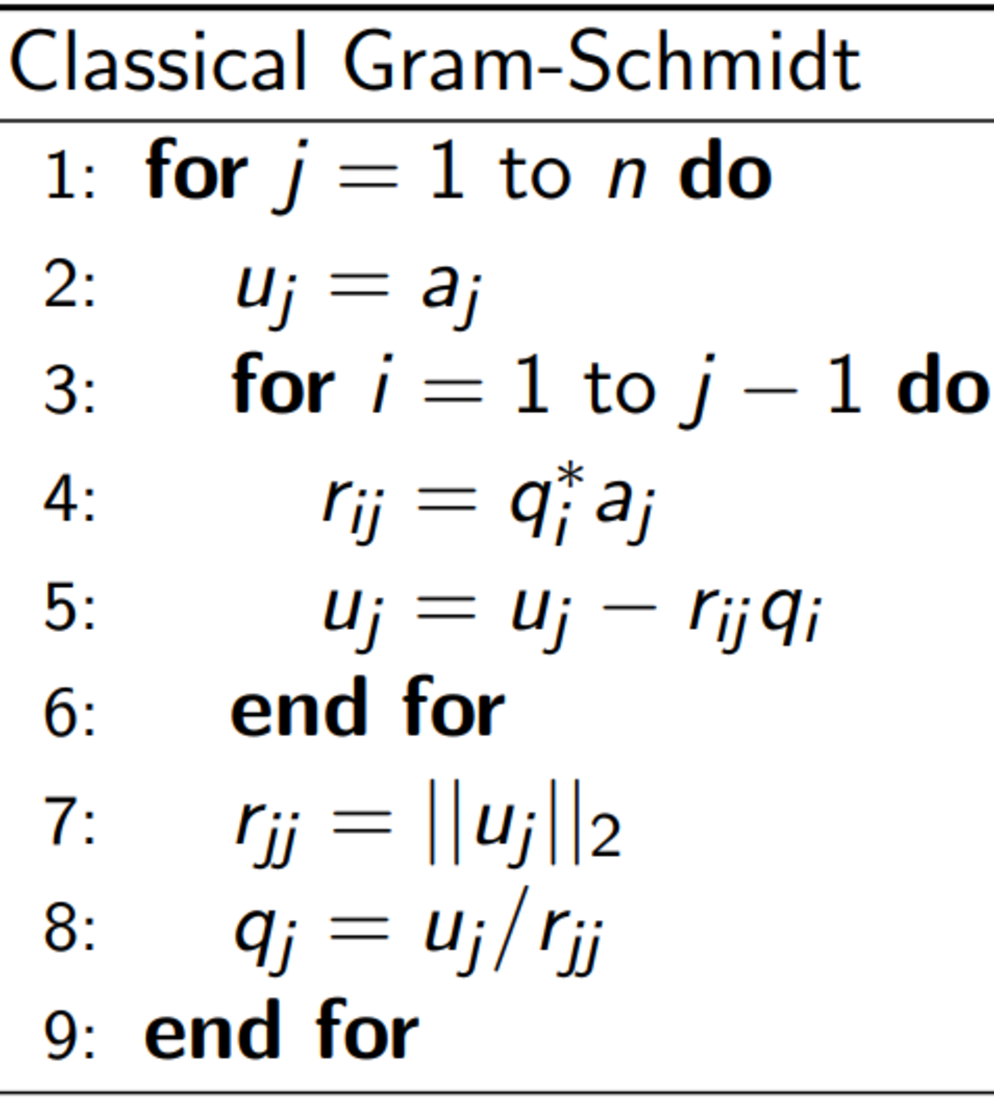
\includegraphics[width=45pt]{classicgm2}
                  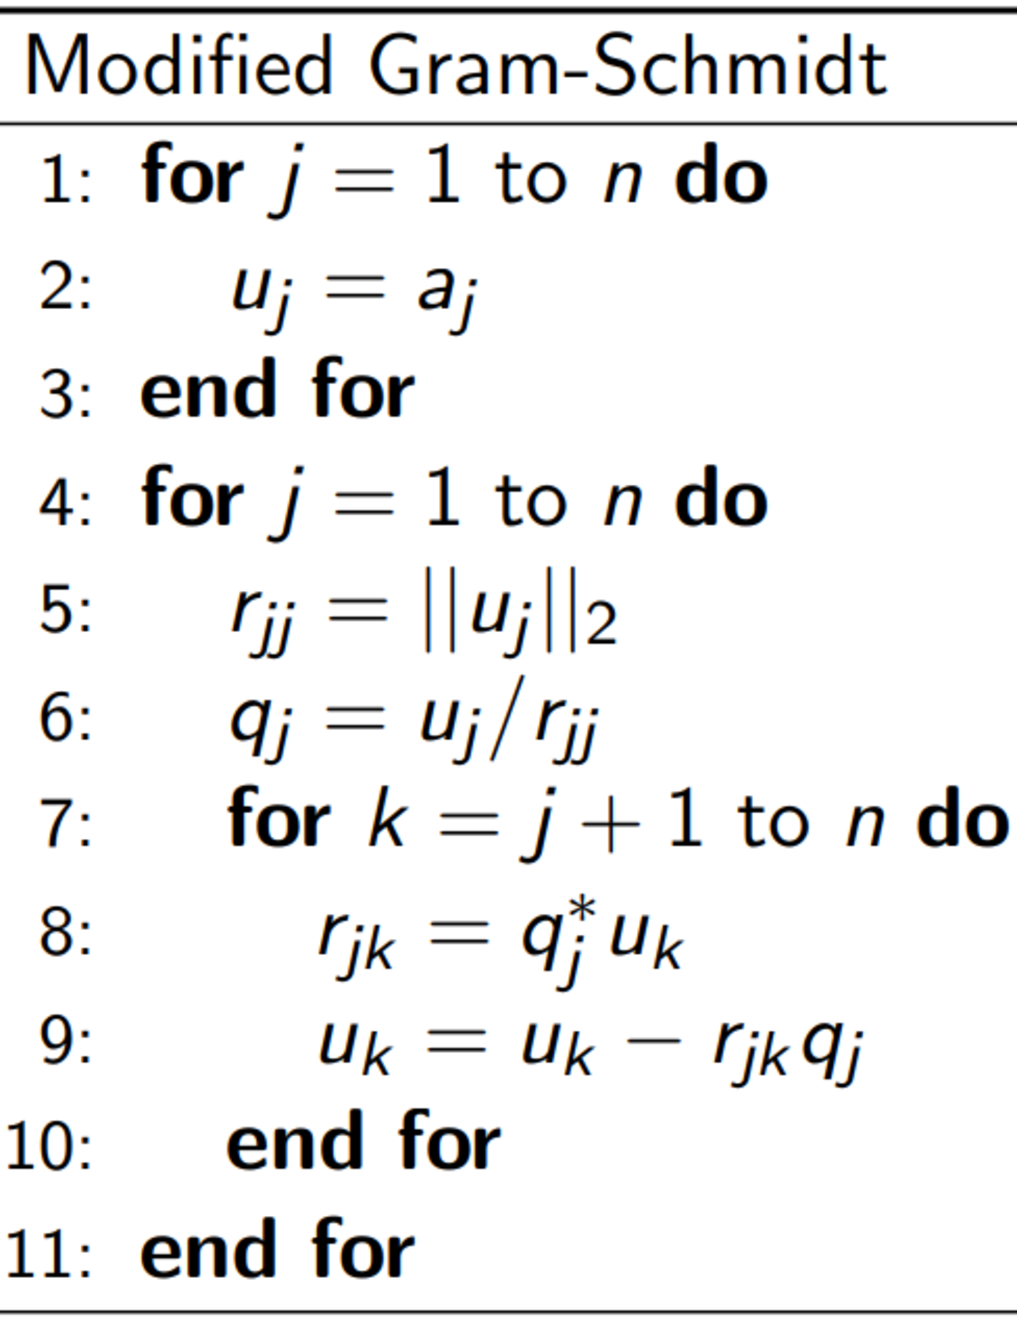
\includegraphics[width=45pt]{modifiedgm2}
            }
      \vItem
            Computes at \iMbox{j}-th step:

            \begin{itemize}

                  \vItem
                        \textbf{Classical GS} => \iMbox{j}-th column of
                        \iMbox{Q} and the \iMbox{j}-th column of \iMbox{R}
                  \vItem
                        \textbf{Modified GS} => \iMbox{j}-th column of
                        \iMbox{Q} and the \iMbox{j}-th row of \iMbox{R}
            \end{itemize}
      \vItem
            Both have \textbf{flop (floating-point operation)} count of
            \iMbox{O(2mn^2)}

            \begin{itemize}

                  \vItem
                        NOTE: \textbf{Householder method} has
                        \iMbox{2\left(m n^2- {n^3} \middle/ {3}\right)} \textbf{flop} count,
                        but better numerical properties
            \end{itemize}
      \vItem
            Recall: \iMbox{\ds Q^{\dagger} Q = \mathbf{I}_{n}} =>
            check for loss of orthogonality with
            \iMbox{\ds \lVert \mathbf{I}_{n} - Q^{\dagger}Q \rVert = \mathrm{loss}}

            \begin{itemize}

                  \vItem
                        \textbf{Classical GS} =>
                        \iMbox{\ds \lVert \mathbf{I}_{n} - Q^{\dagger}Q \rVert \approx \mathrm{Cond}(A)^2\epsilon_{\mathrm{mach}}}
                  \vItem
                        \textbf{Modified GS} =>
                        \iMbox{\ds \lVert \mathbf{I}_{n} - Q^{\dagger}Q \rVert \approx \mathrm{Cond}(A)\epsilon_{\mathrm{mach}}}
                  \vItem
                        NOTE: \textbf{Householder method} has
                        \iMbox{\ds \lVert \mathbf{I}_{n} - Q^{\dagger}Q \rVert \approx \epsilon_{\mathrm{mach}}}
            \end{itemize}
\end{itemize}

\subsection*{Multivariate Calculus}


Consider \iMbox{f: \mathbb{R}^{n} \to \mathbb{R}}:

\begin{itemize}
      \vItem \textbf{When clear} write \textbf{\iMbox{i}-th component} of input as
            \iMbox{i} instead of \iMbox{\mathbf{x}_{i}}

      \vItem \textbf{Level curve} w.r.t. to \iMbox{c \in \mathbb{R}} is all points
            s.t. \iMbox{f(\mathbf{x}) = c}

      \vItem
            Projecting \ul{level curves} onto \iMbox{\mathbb{R}^{n}} gives \iMbox{f}'s \textbf{contour-map}
\end{itemize}

\hSep % ---

\textbf{\iMbox{n_{k}}-th order partial derivative} w.r.t
\iMbox{i_{k}}, of \ldots, of \textbf{\iMbox{n_{1}}-th order partial derivative}
w.r.t \iMbox{i_{1}} of \iMbox{f} is:

\begin{itemize}

      \vItem
            \iMbox{
            \frac{\partial^{n_{k} + \cdots + n_{1}} f}{\partial \mathbf{x}_{i_{k}}^{n_{k}}\cdots\partial \mathbf{x}_{i_{1}}^{n_{1}}} \ = \
            \partial^{n_{k}}_{i_{k}} \cdots \partial^{n_{1}}_{i_{1}} f \ = \  f^{(n_{1},\dots,n_{k})}_{i_{1} \cdots  i_{k}} }
      \vItem
            Its an \textbf{\iMbox{N}-th order partial derivative} where \iMbox{N = \sum_{k} n_{k}}

      \vItem \iMbox{\nabla f = \left[ \partial_{1} f, \dots, \partial_{n} f \right]^{T}}
            is \ul{gradient} of \iMbox{f} => \iMbox{(\nabla f)_{i} = \frac{\partial f}{\partial \mathbf{x}_{i}}}

      \vItem \iMbox{\nabla^{T} f = (\nabla f)^{T}} is \ul{transpose} of \iMbox{\nabla f}, i.e. \iMbox{\nabla^{T}f} is \ul{row vector}
\end{itemize}

\hSep % ---

\iMbox{D_{\mathbf{u}}f(\mathbf{x}) = \lim_{ \delta \to 0 } \frac{f(\mathbf{x} + \delta \mathbf{u}) - f(\mathbf{x})}{\delta}}
is \textbf{directional-derivative} of \iMbox{f}
\begin{itemize}

      \vItem
            It is \ul{rate-of-change} in direction \iMbox{\mathbf{u}}, where \iMbox{\mathbf{u} \in \mathbb{R}^{n}} is \ul{unit-vector}
      \vItem
            \iMbox{D_{\mathbf{u}}f(\mathbf{x}) = \nabla f(\mathbf{x}) \cdot \mathbf{u} = \lVert \nabla f(\mathbf{x}) \rVert \lVert \mathbf{u} \rVert \cos(\theta)}
            => \iMbox{D_{\mathbf{u}}f(\mathbf{x})} \textbf{maximized} when \iMbox{\cos\theta = 1}
      \vItem
            i.e. when \iMbox{\mathbf{x},\mathbf{u}} are \ul{parallel} => hence \iMbox{\nabla f(\mathbf{x})} is
            \ul{direction} of \textbf{max.} \ul{rate-of-change}
\end{itemize}

\hSep % ---

\iMbox{f} has \textbf{local minimum} at \iMbox{\mathbf{x}_{\mathrm{loc}}} if there's radius \iMbox{r>0}
s.t. \iMbox{\forall \mathbf{x} \in B[r;\mathbf{x}_{\mathrm{loc}}]} we have \iMbox{f(\mathbf{x}_{\mathrm{loc}}) \leq f(\mathbf{x})}

\iMbox{f} has \textbf{global minimum} \iMbox{\mathbf{x}_{\mathrm{glob}}} if \iMbox{\forall \mathbf{x} \in \mathbb{R}^{n}}
we have \iMbox{f(\mathbf{x}_{\mathrm{glob}}) \leq f(\mathbf{x})}

A \textbf{local minimum} satisfies \ul{optimality conditions}:
\begin{itemize}
      \vItem
            \iMbox{\nabla f(\mathbf{x}) = \mathbf{0}}, e.g.~for \iMbox{n=1}
            its \iMbox{f'(x) = 0}
      \vItem
            \iMbox{\nabla^2 f(\mathbf{x})} is \ul{positive-definite},
            e.g. for \iMbox{n=1} its \iMbox{f''(x) > 0}
\end{itemize}

\hSep % ---

\iMbox{\mathbf{H}(f) = \nabla^2 f = \mathbf{J}(\nabla f)^{T}} is \textbf{\emph{Hessian}} =>
\iMbox{\mathbf{H}(f)_{ij} = \frac{\partial^2 f}{\partial \mathbf{x}_{i}\partial \mathbf{x}_{j}}}

Interpret \iMbox{F: \mathbb{R}^n \to \mathbb{R}^{m}} as \iMbox{m} functions \iMbox{F_{i}: \mathbb{R}^{n} \to \mathbb{R}}
\emph{(one per output-component)}
\begin{itemize}
      \vItem
            \iMbox{\mathbf{J}(F) = \left[ \nabla^{T} F_{1}; \ \dots; \ \nabla^{T} F_{m} \right]}
            is \textbf{\emph{Jacobian}} =>
            \iMbox{\mathbf{J}(F)_{ij} = \frac{\partial F_i}{\partial \mathbf{x}_j}}
\end{itemize}


\subsection*{Conditioning}

A \textbf{\emph{problem}} is some \iMbox{f:X \to Y} where \iMbox{X,Y}
are normed vector-spaces

\begin{itemize}

      \vItem
            A problem \textbf{\emph{instance}} is \iMbox{f} with fixed input
            \iMbox{x \in X}, shortened to \textbf{\emph{just}} \ul{``problem''}
            (with \iMbox{x \in X} implied)
      \vItem
            \iMbox{\delta x} is \textbf{small perturbation} of \iMbox{x}
            => \iMbox{\delta f = f(x+\delta x)-f(x)}
\end{itemize}

A \ul{problem (instance)} is:
\begin{itemize}

      \vItem
            \textbf{Well-conditioned} if \ul{all} \textbf{small} \iMbox{\delta x}
            lead to \textbf{small} \iMbox{\delta f}, i.e. if \iMbox{\kappa} is
            \textbf{small} \emph{(e.g. \iMbox{1}, \iMbox{10}, \iMbox{10^{2}})}
      \vItem
            \textbf{Ill-conditioned} if \ul{some} \textbf{small} \iMbox{\delta x}
            lead to \textbf{large} \iMbox{\delta f}, i.e. if \iMbox{\kappa} is
            \textbf{large} \emph{(e.g. \iMbox{10^6}, \iMbox{10^{16}})}
\end{itemize}

\hSep % ---

\textbf{\emph{Absolute} condition number} \iMbox{\mathrm{cond}(x) = \hat{\kappa}(x) = \hat{\kappa}}
of \textbf{\iMbox{f} at \iMbox{x}}:
\begin{itemize}

      \vItem
            \iMbox{ \hat{\kappa}=\lim _{\delta \rightarrow 0} \sup _{\|\delta x\| \leq \delta} \frac{\|\delta f\|}{\|\delta x\|}}

            => for \ul{most problems} simplified to
            \iMbox{\hat{\kappa}=\sup _{\delta x} \frac{\|\delta f\|}{\|\delta x\|}}
      \vItem
            If \ul{Jacobian} \iMbox{\mathbf{J}_{f}(x)} exists then \iMbox{\hat{\kappa} = \lVert \mathbf{J}_{f}(x) \rVert},
            where \ul{matrix norm} \iMbox{\lVert - \rVert} induced by \ul{norms} on \iMbox{X} and \iMbox{Y}
\end{itemize}

\textbf{\emph{Relative} condition number} \iMbox{\kappa(x) = \kappa} of \textbf{\iMbox{f} at \iMbox{x}} is
\begin{itemize}

      \vItem
            \iMbox{\kappa=\lim _{\delta \rightarrow 0} \sup _{\|\delta x\| \leq \delta}\left(\frac{\|\delta f\|}{\|f(x)\|} \middle/ \frac{\|\delta x\|}{\|x\|}\right)}

            => for \ul{most problems} simplified to
            \iMbox{\kappa=\sup _{\delta x}\left(\frac{\|\delta f\|}{\|f(x)\|} \middle/ \frac{\|\delta x\|}{\|x\|}\right)}
      \vItem
            If \ul{Jacobian} \iMbox{\mathbf{J}_{f}(x)} exists then
            \iMbox{\kappa=\frac{\|\mathbf{J}_{f}(x)\|}{\|f(x)\| /\|x\|}}
      \vItem
            \ul{More important} than \iMbox{\hat{\kappa}} for \emph{numerical analysis}
\end{itemize}

\textbf{\emph{Matrix} condition number} \iMbox{\mathrm{Cond}(\mathbf{A}) = \kappa(\mathbf{A}) = \lVert \mathbf{A} \rVert \lVert \mathbf{A}^{-1} \rVert}
=> comes up \ul{so often} that has \ul{its own name}
\begin{itemize}
      \vItem
            \iMbox{\mathbf{A} \in \mathbb{C}^{m \times m}} is \ul{well-conditioned} if
            \iMbox{\kappa(\mathbf{A})} is \textbf{small}, \ul{ill-conditioned} if
            \textbf{large}
      \vItem
            \iMbox{\kappa(\mathbf{A}) = \kappa(\mathbf{A}^{-1})}
            \iMbox{\kappa(\mathbf{A}) = \kappa(\gamma \mathbf{A})}
            \iMbox{\lVert \cdot \rVert = {\lVert \cdot \rVert}_{2} \implies \kappa(\mathbf{A}) = \frac{\sigma_{1}}{\sigma_{m}}}
\end{itemize}

\hSep % ---

For \iMbox{\mathbf{A} \in \mathbb{C}^{m \times n}}, the problem
\iMbox{f_{\mathbf{A}}(x) = \mathbf{A}x} has
\iMbox{\kappa=\|\mathbf{A}\| \frac{\|x\|}{\|\mathbf{A} x\|}} => if
\iMbox{\mathbf{A}^{-1}} exists then \iMbox{\kappa \leq \mathrm{Cond}(\mathbf{A})}

\begin{itemize}

      \vItem
            If \iMbox{\mathbf{A}x = b}, problem of finding \iMbox{x} given \iMbox{b} is
            just \iMbox{f_{\mathbf{A}^{-1}}(b) = \mathbf{A}^{-1}b} =>
            \iMbox{\kappa=\left\|\mathbf{A}^{-1}\right\| \frac{\|b\|}{\|x\|} \leq \mathrm{Cond}(\mathbf{A})}
\end{itemize}

For \iMbox{\mathbf{b} \in \mathbb{C}^{m}}, the problem
\iMbox{f_{\mathbf{b}}(A) = A^{-1}\mathbf{b}} \emph{(i.e.~finding
      \iMbox{x} in \iMbox{Ax = \mathbf{b}})} has
\iMbox{\kappa=\|A\|\left\|A^{-1}\right\|=\mathrm{Cond}(A)}


\subsection*{Stability}

Given a \ul{problem} \iMbox{f: X \to Y}, an \textbf{algorithm} for
\iMbox{f} is \iMbox{\tilde{f}: X  \to Y}

\begin{itemize}
      \vItem
            Input \iMbox{x \in X} is first \ul{rounded} to \iMbox{\mathrm{fl}(x)},
            i.e. \iMbox{\tilde{f}(x) = \tilde{f}\left(\mathrm{fl}\left(x \right) \right)}
      \vItem
            \textbf{Absolute error} => \iMbox{\|\tilde{f}(x)-f(x)\|};

            \textbf{relative error} => \iMbox{\frac{\|\tilde{f}(x)-f(x)\|}{\|f(x)\|}}
\end{itemize}

\iMbox{\tilde{f}} is \textbf{accurate} if \iMbox{\forall x \in X},
\iMbox{\frac{\|\tilde{f}(x)-f(x)\|}{\|f(x)\|}=O\left(\epsilon_{\mathrm{mach}}\right)}

\iMbox{\tilde{f}} is \textbf{stable} if \iMbox{\forall x \in X},
\iMbox{\exists \tilde{x} \in X} s.t.
\iMbox{\frac{\|\tilde{f}(x)-f( \tilde{x})\|}{\|f( \tilde{x})\|}=O\left(\epsilon_{\mathrm{mach}}\right)}
and
\iMbox{\frac{\|\tilde{x}-x\|}{\|x\|}=O\left(\epsilon_{\mathrm{mach}}\right)}

\begin{itemize}

      \vItem
            i.e. \ul{nearly} the right answer to \ul{nearly} the right question
      \vItem
            \textbf{outer-product} is stable
\end{itemize}

\columnbreak

\iMbox{\tilde{f}} is \textbf{backwards stable} if
\iMbox{\forall x \in X}, \iMbox{\exists \tilde{x} \in X} s.t.
\iMbox{\tilde{f}(x) = f(\tilde{x})} and
\iMbox{\frac{\|\tilde{x}-x\|}{\|x\|}=O\left(\epsilon_{\mathrm{mach}}\right)}

\begin{itemize}

      \vItem
            i.e. \ul{exactly} the right answer to \ul{nearly} the right question,
            a \textbf{subset of stability}
      \vItem
            \iMbox{\oplus, \ominus, \otimes, \oslash}, \textbf{inner-product},
            back-substitution w/ triangular systems, are \ul{backwards stable}
      \vItem
            If \textbf{backwards stable} \iMbox{\tilde{f}} and \iMbox{f} has
            \ul{condition number} \iMbox{\kappa(x)} then \ul{relative error}
            \iMbox{\frac{\|\tilde{f}(x)-f(x)\|}{\|f(x)\|} = O\left(\kappa(x)\epsilon_{\mathrm{mach}}\right)}
\end{itemize}

\ul{Accuracy, stability, backwards stability} are \textbf{norm-independent} for fin-dim \iMbox{X,Y}

\subsection*{Big-O meaning for numerical analysis}

In \ul{complexity analysis} \iMbox{f(n)=O(g(n))} as \iMbox{n \to \infty}

But in \ul{numerical analysis} \iMbox{f(\epsilon)=O(g(\epsilon))} as \iMbox{\epsilon \to 0},
i.e. \iMbox{\limsup_{\epsilon \to 0} \left. {\lVert f(\epsilon) \rVert} \ \middle/ \ {\lVert g(\epsilon) \rVert} \right. < \infty}

\begin{itemize}
      \vItem
            i.e. \iMbox{\exists C,\delta>0} s.t. \iMbox{\forall \epsilon}, we have
            \iMbox{0 < \lVert \epsilon \rVert<\delta \implies \lVert f(\epsilon) \rVert \leq C \lVert g(\epsilon) \rVert}
      \vItem
            \iMbox{O(g)} is \ul{set of functions}
            \iMbox{\{ f \ \ : \ \ \limsup_{\epsilon \to 0} \left. {\lVert f(\epsilon) \rVert} \ \middle/ \ {\lVert g(\epsilon) \rVert} \right. < \infty \}}
\end{itemize}

\hSep % ---

\textbf{Smallness} \ul{partial order} \iMbox{\ds O(g_{1}) \preceq O(g_{2})}
defined by \ul{set-inclusion} \iMbox{\ds O(g_{1}) \subseteq O(g_{2})}

\begin{itemize}

      \vItem
            i.e. as \iMbox{\epsilon \to 0}, \iMbox{g_{1}(\epsilon)} \ul{goes to zero}
            \textbf{\emph{faster}} than \iMbox{g_{2}(\epsilon)}
      \vItem
            \emph{Roughly} same \ul{hierarchy} as \ul{complexity analysis} but
            \textbf{flipped} \emph{(some don't fit the pattern)}

            \begin{itemize}
                  \vItem e.g. \iMbox{\dots, O(\epsilon^3) \prec O(\epsilon^2) \prec O(\epsilon) \prec O(1)}
            \end{itemize}
      \vItem
            \textbf{Maximum}:
            \iMbox{O(\max(\lvert g_{1} \rvert, \lvert g_{2} \rvert))=O(g_{2}) \iff O(g_{1}) \preceq O(g_{2})}

            \begin{itemize}
                  \vItem e.g. \iMbox{O(\max(\epsilon^{k}, \epsilon))=O(\epsilon)}
            \end{itemize}
\end{itemize}

\hSep % ---

Using \ul{functions} \iMbox{f_{1},\dots,f_{n}}, let \iMbox{\mathbfit{\Phi}(f_{1},\dots,f_{n})}
be \ul{formula} \textbf{defining some function}

\begin{itemize}

      \vItem
            Then \iMbox{\mathbfit{\Phi}(O(g_{1}),\dots,O(g_{n}))} is the \ul{class of functions}
            \iMbox{\left\{ \mathbfit{\Phi}(f_{1},\dots,f_{n}) \ \ : \ \ f_{1} \in O(g_{1}),\dots,f_{n} \in O(g_{n}) \right\}}
            \begin{itemize}
                  \vItem
                        e.g. \iMbox{\epsilon^{O(1)} = \{ \epsilon^{f(\epsilon)} : f \in O(1) \}}
            \end{itemize}
      \vItem
            \ul{General case}:
            \iMbox{\mathbfit{\Phi}_{1}(O(f_{1}),\dots,O(f_{m})) = \mathbfit{\Phi}_{2}(O(g_{1}),\dots,O(g_{n}))}
            means
            \iMbox{\mathbfit{\Phi}_{1}(O(f_{1}),\dots,O(f_{m})) \subseteq \mathbfit{\Phi}_{2}(O(g_{1}),\dots,O(g_{n}))}

            \begin{itemize}
                  \vItem
                        e.g. \iMbox{\epsilon^{O(1)} = O\left(k^{\epsilon}\right)}
                        means
                        \iMbox{\{ \epsilon^{f(\epsilon)} : f \in O(1) \} \subseteq O\left(k^{\epsilon}\right)};
                        \emph{not necessarily true}
            \end{itemize}
      \vItem
            \ul{Special case}: \iMbox{f = \mathbfit{\Phi}(O(g_{1}),\dots,O(g_{n}))}
            means \iMbox{f \in \mathbfit{\Phi}(O(g_{1}),\dots,O(g_{n}))}
            \begin{itemize}
                  \vItem
                        e.g. \iMbox{(\epsilon+1)^2 = \epsilon^2 + O(\epsilon)} means
                        \iMbox{{\epsilon \mapsto (\epsilon+1)^2} \ \in \ \{ \epsilon^2 + f(\epsilon) : f \in O(\epsilon) \}};
                        \emph{not necessarily true}
            \end{itemize}
\end{itemize}

\hSep % ---

Let \iMbox{f_{1} = O(g_{1}), \ f_{2} = O(g_{2})} and let \iMbox{k \neq 0} be a \ul{constant}

\begin{itemize}

      \vItem
            \iMbox{f_{1}f_{2} = O(g_{1}g_{2})}; \iMbox{f \cdot O(g) = O(fg)}; \iMbox{O(\lvert k \rvert \cdot g) = O(g)}
      \vItem
            \iMbox{f_{1} + f_{2} = O(\max(\lvert g_{1} \rvert, \lvert g_{2} \rvert))}

            => \textbf{if} \iMbox{g_{1} = g = g_{2}} \textbf{then} \iMbox{f_{1}+f_{2} = O(g)}
\end{itemize}


\subsection*{Floating-point numbers}

Consider \textbf{base/radix} \iMbox{\beta\geq 2} \emph{(typically
      \iMbox{2})} and \textbf{precision} \iMbox{t\geq 1} \emph{(\iMbox{24}
      or \iMbox{53} for IEEE single/double precisions)}

\textbf{Floating-point numbers} are discrete subset
\iMbox{\mathbf{F} = \left\{ \ (-1)^{s} \left(m \middle/ \beta^t\right) \beta^e \ \middle| \ 1 \leq m \leq \beta^t, \ s \in \mathbb{B}, m,e \in \mathbb{Z} \ \right\}}
\begin{itemize}

      \vItem
            \iMbox{s} is \textbf{sign-bit}, \iMbox{m / \beta^t} is
            \textbf{mantissa}, \iMbox{e} is \textbf{exponent}
            \emph{(\iMbox{8}-bit for single, \iMbox{11}-bit for double)}
      \vItem
            Equivalently, can restrict to
            \iMbox{\beta^{t-1} \leq m \leq \beta^t-1} for \ul{unique} \iMbox{m} and
            \iMbox{e}
      \vItem
            \iMbox{\mathbf{F}\subset \mathbb{R}} is \ul{idealized} 
            \emph{(ignores over/underflow)}, so is \ul{countably infinite} and \ul{self-similar}
            \emph{(i.e. \iMbox{\mathbf{F} = \beta \mathbf{F}})}
      \vItem
            For all \iMbox{x \in \mathbb{R}} there exists \iMbox{\mathrm{fl}(x) \in \mathbf{F}} s.t.
            \iMbox{\lvert x - \mathrm{fl}(x) \rvert \leq \epsilon_{\mathrm{mach}} \lvert x \rvert}

            \begin{itemize}
                  \vItem
                        Equivalently
                        \iMbox{\mathrm{fl}(x) = x(1 + \delta), \lvert \delta \rvert \leq \epsilon_{\mathrm{mach}}}
            \end{itemize}
\end{itemize}

\textbf{Machine epsilon}
\iMbox{\epsilon_{\mathrm{machine}} = \epsilon_{\mathrm{mach}} = \frac{1}{2}\beta^{1-t}}
\ul{is maximum relative gap between FPs}
\begin{itemize}
      \vItem
            \ul{Half the gap} between \iMbox{1} and \ul{next largest FP}
      \vItem
            \iMbox{2^{-24} \approx 5.96 \times 10^{-8}} and
            \iMbox{2^{-53} \approx 10^{-16}} for single/double
\end{itemize}

\hSep % ---

\textbf{FP arithmetic}: let \iMbox{\ast, \circledast} be \ul{real} and
\ul{floating} counterparts of \ul{arithmetic operation}

\begin{itemize}
      \vItem
            For \iMbox{x,y \in \mathbf{F}} we have
            \iMbox{x \circledast y = \mathrm{fl}(x \ast y) = (x * y)(1+\epsilon), \lvert \delta \rvert \leq \epsilon_{\mathrm{mach}}}

            \begin{itemize}
                  \vItem
                        Holds for \textbf{\emph{any}} \ul{arithmetic operation}
                        \iMbox{\circledast = \oplus, \ominus, \otimes, \oslash}
            \end{itemize}
      \vItem
            \ul{Complex floats} implemented \ul{pairs of real floats}, so above applies
            to \ul{complex ops} as-well

            \begin{itemize}
                  \vItem
                        \ul{Caveat:} \iMbox{\epsilon_{\mathrm{mach}} = \frac{1}{2}\beta^{1-t}}
                        must be \ul{scaled} by factors \ul{on the order of} \iMbox{2^{3/2},2^{5/2}}
                        for \iMbox{\otimes, \oslash} \emph{respectively}
            \end{itemize}
      \vItem
            \iMbox{
                  \begin{aligned}
                        (x_{1} \oplus \dots &\oplus x_{n}) 
                        \\ &\approx (x_{1} + \dots +x_{n}) + \sum_{i=1}^{n} x_{i}\left( \sum_{j=i}^{n} \delta_{j} \right)
                  \end{aligned}
                  ; \ \lvert \delta_{j} \rvert \leq \epsilon_{\mathrm{mach}}
            }
      \vItem
            \iMbox{(x_{1} \otimes \dots \otimes x_{n}) \approx (x_{1} \times \dots \times x_{n})(1+\epsilon), \epsilon \leq 1.06(n-1)\epsilon_{\mathrm{mach}}}
      \vItem
            \iMbox{\mathrm{fl}\left( \sum x_{i} y_{i} \right) = \sum x_{i}y_{i}(1 + \epsilon_{i})}
            where
            \iMbox{1+ \epsilon_{i} = (1+ \delta_{i}) \times(1 + \eta_{i}) \cdots (1 + \eta_{n})}
            and
            \iMbox{\lvert \delta_{j} \rvert, \lvert \eta_{i} \rvert \leq \epsilon_{\mathrm{mach}}}

            \begin{itemize}

                  \vItem
                        \iMbox{1+ \epsilon_{i} \approx 1 + \delta_{i} + (\eta_{i} + \dots + \eta_{n})}
                  \vItem
                        \iMbox{|\mathrm{fl}(x^T y) - x^T y| \leq \sum \lvert x_{i} y_{i} \rvert \lvert \epsilon_{i} \rvert}
                  \vItem
                        Assuming \iMbox{n \epsilon_{\mathrm{mach}} \leq 0.1}
                        =>
                        \iMbox{|\mathrm{fl}(x^T y) - x^T y| \leq \phi(n) \epsilon_{\mathrm{mach}} \lvert x \rvert^T \lvert y \rvert},
                        where \iMbox{\lvert x \rvert_{i} = \lvert x_{i} \rvert} is \ul{vector}
                        and \iMbox{\phi(n)} is \ul{small function} of \iMbox{n}
            \end{itemize}
      \vItem
            \textbf{Summing a series} is \ul{more stable} if terms \ul{added in order of increasing magnitude}
\end{itemize}

\columnbreak

For \textbf{FP matrices}, let
\iMbox{\lvert M \rvert_{ij} = \lvert M_{ij} \rvert}, i.e. matrix
\iMbox{\lvert M \rvert} of \ul{absolute values} of \iMbox{M}
\begin{itemize}

      \vItem
            \iMbox{\mathrm{fl}(\lambda \mathbf{A}) = \lambda \mathbf{A} + E; \lvert E \rvert_{ij} \leq \lvert \lambda \mathbf{A} \rvert_{ij} \epsilon_{\mathrm{mach}}}
      \vItem
            \iMbox{\mathrm{fl}(\mathbf{A} + \mathbf{B}) = (\mathbf{A} + \mathbf{B}) + E; \lvert E \rvert_{ij} \leq \lvert \mathbf{A} + \mathbf{B} \rvert_{ij} \epsilon_{\mathrm{mach}}}
      \vItem
            \iMbox{\mathrm{fl}(\mathbf{A}\mathbf{B}) = \mathbf{A}\mathbf{B} + E; \lvert E \rvert_{ij} \leq n 
            \epsilon_{\mathrm{mach}}(\lvert \mathbf{A} \rvert \lvert \mathbf{B} \rvert)_{ij} + O\left({\epsilon_{\mathrm{mach}}}^{2} \right)}
\end{itemize}

\hSep % ---

\textbf{\emph{Taylor series}} about \iMbox{a\in \mathbb{R}} is
\iMbox{f(x)=\sum_{k=0}^n \frac{f^{(k)}(a)}{k!}(x-a)^k + O\left((x-a)^{n+1}\right)}
as \iMbox{x \to a}

\begin{itemize}

      \vItem
            Need \iMbox{a=0} => \iMbox{f(x)=\sum_{k=0}^n \frac{f^{(k)}(0)}{k!}x^k + O\left(x^{n+1}\right)}
            as \iMbox{x \to 0}
      \vItem
            e.g.\iMbox{(1+\epsilon)^p = \begin{aligned}
                  &\sum_{k=0}^n {\binom{p}{k}\epsilon^{k}} + O\left(\epsilon^{n+1}\right) 
                  \\ &= \sum_{k=0}^n \frac{p!}{k!(p-k)!}\epsilon^{k} + O\left(\epsilon^{n+1}\right)
            \end{aligned}} as \iMbox{\epsilon \to 0}
\end{itemize}
